\chapter{BÀI TOÁN, DỮ LIỆU VÀ TIỀN XỬ LÝ}
\label{chap:data}

Chương này phát biểu bài toán học máy của đề tài, mô tả bộ dữ liệu, trình bày kết quả khảo sát dữ liệu, các vấn đề chất lượng dữ liệu cùng cách xử lý, và quy trình chuẩn bị dữ liệu cho mô hình.

\section{Phát biểu bài toán}
\label{sec:problem}

\subsection{Bài toán học máy}
Đề tài dự báo điện năng tiêu thụ trong một giờ của hộ gia đình, dựa trên dữ liệu đo trong quá khứ. Bảng~\ref{tab:problem} cụ thể hóa bài toán trên dữ liệu của nhóm.

\begin{table}[htbp]
    \centering
    \caption{Phát biểu bài toán học máy.}
    \label{tab:problem}
    \small
    \begin{tabularx}{\textwidth}{|>{\raggedright\arraybackslash}p{3.0cm}|>{\raggedright\arraybackslash}X|}
        \hline
        \textbf{Thành phần} & \textbf{Nội dung} \\ \hline
        Loại bài toán & Học có giám sát, hồi quy: đầu ra là một số thực liên tục. \\ \hline
        Đơn vị mẫu & Một cặp (thời điểm gốc $t$ theo giờ, tầm dự báo $h$). Ví dụ: lúc 20:00 ngày 03/02/2009 dùng dữ liệu đến 20:00 để dự báo điện năng của giờ 21:00 ($h = 1$). \\ \hline
        Đầu ra & $y_{t+h}$: điện năng tiêu thụ trong giờ $t+h$ (kWh), tính từ công suất đo theo phút (Mục~\ref{sec:label}). \\ \hline
        Đầu vào & Chỉ gồm thông tin biết được tại $t$: điện năng các giờ trước, thống kê cửa sổ trượt và lịch của thời điểm mục tiêu (21 đặc trưng, Mục~\ref{sec:features}). \\ \hline
        Tầm dự báo & $h \in \{1, 6, 12, 24\}$ giờ, mỗi $h$ một mô hình (chiến lược trực tiếp). \\ \hline
        Số mẫu có nhãn & Huấn luyện (nhãn trước 01/01/2010): 26.523 ($h=1$) đến 26.500 ($h=24$); kiểm tra (năm 2010): 7.620. \\ \hline
    \end{tabularx}
\end{table}

\subsection{Mục tiêu và tiêu chí thành công}
Bảng~\ref{tab:objectives} chuyển mục tiêu thực tế thành mục tiêu học máy và chỉ số đo.

\begin{table}[htbp]
    \centering
    \caption{Mục tiêu thực tế, mục tiêu học máy và chỉ số đánh giá.}
    \label{tab:objectives}
    \small
    \begin{tabularx}{\textwidth}{|>{\raggedright\arraybackslash}p{3.6cm}|>{\raggedright\arraybackslash}p{3.8cm}|>{\raggedright\arraybackslash}X|}
        \hline
        \textbf{Mục tiêu thực tế} & \textbf{Mục tiêu học máy} & \textbf{Chỉ số và mức kết quả} \\ \hline
        Biết trước mức tiêu thụ trong 1--24 giờ tới & Dự báo $y_{t+h}$ với sai số tuyệt đối nhỏ & Chỉ số chính: MAE (kWh). Mức tham chiếu: MAE của mô hình cơ sở tốt nhất trên kiểm định chéo. Mức mong muốn (nhóm tự đặt): giảm ít nhất 10\% so với mức tham chiếu ở mọi $h$. \\ \hline
        Không bỏ sót giờ cao điểm & Hạn chế sai số lớn & RMSE (phạt nặng sai số lớn); phân tích sai số theo giờ trong ngày. \\ \hline
        Dễ trình bày cho người dùng & Có thước đo tương đối & MAPE, chỉ để tham khảo vì nhiều giờ có điện năng rất nhỏ. \\ \hline
        Kết quả tin cậy & Đánh giá không rò rỉ, đủ ổn định & Trung bình $\pm$ độ lệch chuẩn qua 5 fold TimeSeriesSplit; tập kiểm tra chỉ dùng một lần ở cuối. \\ \hline
    \end{tabularx}
\end{table}

MAE được chọn làm chỉ số chính vì có đơn vị kWh dễ diễn giải, và vì nhãn lệch phải với một số ít giờ đỉnh (Mục~\ref{sec:label}): MAE ít bị các giờ đỉnh chi phối hơn RMSE. MAPE không dùng làm chỉ số chính vì nhãn có giá trị nhỏ nhất chỉ 0,124 kWh, khiến sai số phần trăm bị phóng đại ở các giờ tải nền~\cite{hyndman2021fpp3,hyndman2006another}.

\section{Dữ liệu}
\label{sec:dataset}

\subsection{Nguồn và điều kiện sử dụng}
Bảng~\ref{tab:source} tóm tắt thông tin bộ dữ liệu. Dữ liệu có giấy phép CC BY 4.0, cho phép sử dụng và chia sẻ với điều kiện ghi nguồn.

\begin{table}[htbp]
    \centering
    \caption{Thông tin bộ dữ liệu.}
    \label{tab:source}
    \small
    \begin{tabularx}{\textwidth}{|>{\raggedright\arraybackslash}p{3.6cm}|>{\raggedright\arraybackslash}X|}
        \hline
        \textbf{Thuộc tính} & \textbf{Giá trị} \\ \hline
        Tên, nguồn & \textit{Individual Household Electric Power Consumption}, UCI Machine Learning Repository~\cite{hebrail2006uci} \\ \hline
        DOI, giấy phép & 10.24432/C58K54; Creative Commons Attribution 4.0 \\ \hline
        Đối tượng đo & Một hộ gia đình ở Sceaux (cách Paris khoảng 7 km, Pháp) \\ \hline
        Thời gian, tần suất & 16/12/2006 17:24 -- 26/11/2010 21:02; mỗi phút một bản ghi \\ \hline
        Quy mô & 2.075.259 dòng $\times$ 9 cột (2 cột thời gian, 7 biến đo); tệp văn bản phân tách bằng ``;'' \\ \hline
    \end{tabularx}
\end{table}

\subsection{Từ điển dữ liệu}
Bảng~\ref{tab:dictionary} mô tả các cột của dữ liệu gốc. Ý nghĩa và đơn vị lấy theo mô tả của UCI~\cite{hebrail2006uci}; miền giá trị do nhóm đo trên dữ liệu. UCI ghi đơn vị công suất phản kháng là kilowatt; về vật lý đơn vị đúng là kvar nên báo cáo dùng kvar.

\begin{table}[htbp]
    \centering
    \caption{Từ điển dữ liệu của 9 cột gốc.}
    \label{tab:dictionary}
    \small
    \begin{tabularx}{\textwidth}{|>{\raggedright\arraybackslash}p{4.6cm}|>{\raggedright\arraybackslash}X|>{\centering\arraybackslash}p{1.5cm}|>{\raggedright\arraybackslash}p{3.3cm}|}
        \hline
        \textbf{Cột} & \textbf{Ý nghĩa} & \textbf{Đơn vị} & \textbf{Miền giá trị; vai trò} \\ \hline
        \code{Date}, \code{Time} & Ngày (dd/mm/yyyy) và giờ (hh:mm:ss) đo & -- & Ghép thành chỉ mục thời gian \\ \hline
        \code{Global_active_power} & Công suất tác dụng trung bình phút của cả hộ & kW & 0,076--11,122; nguồn của nhãn \\ \hline
        \code{Global_reactive_power} & Công suất phản kháng trung bình phút & kvar & 0--1,390; chỉ dùng khảo sát \\ \hline
        \code{Voltage} & Điện áp trung bình phút & V & 223,20--254,15; không dùng làm đầu vào \\ \hline
        \code{Global_intensity} & Cường độ dòng điện trung bình phút & A & 0,2--48,4; loại bỏ (rò rỉ) \\ \hline
        \code{Sub_metering_1} & Điện năng khu bếp (máy rửa bát, lò nướng, lò vi sóng) & Wh/phút & 0--88; chỉ dùng khảo sát \\ \hline
        \code{Sub_metering_2} & Điện năng phòng giặt (máy giặt, máy sấy, tủ lạnh, đèn) & Wh/phút & 0--80; chỉ dùng khảo sát \\ \hline
        \code{Sub_metering_3} & Điện năng bình nước nóng và điều hòa & Wh/phút & 0--31; chỉ dùng khảo sát \\ \hline
    \end{tabularx}
\end{table}

Khi đọc tệp gốc mà không khai báo giá trị thiếu, sáu cột số từ \code{Global_active_power} đến \code{Sub_metering_2} bị đọc thành chuỗi vì chứa ký tự ``?'' (tổng cộng 155.874 ký tự); riêng \code{Sub_metering_3} để trống ô nên vẫn là số. Nhóm đọc lại dữ liệu, khai báo ``?'' và ô trống là giá trị thiếu, ép kiểu số thực và ghép hai cột thời gian thành chỉ mục.

\section{Khảo sát dữ liệu}
\label{sec:eda}

\subsection{Thống kê mô tả}
Bảng~\ref{tab:describe} là thống kê mô tả của bảy biến đo theo phút.

\begin{table}[htbp]
    \centering
    \caption{Thống kê mô tả bảy biến đo theo phút (2.049.280 giá trị đo mỗi biến).}
    \label{tab:describe}
    \small
    \begin{tabular}{|l|r|r|r|r|r|r|r|}
        \hline
        \textbf{Biến} & \textbf{TB} & \textbf{ĐLC} & \textbf{Min} & \textbf{Trung vị} & \textbf{Max} & \textbf{Skew} & \textbf{\% bằng 0} \\ \hline
        GAP (kW) & 1,092 & 1,057 & 0,076 & 0,602 & 11,122 & 1,79 & 0 \\ \hline
        Reactive (kvar) & 0,124 & 0,113 & 0 & 0,100 & 1,390 & 1,26 & 23,50 \\ \hline
        Voltage (V) & 240,84 & 3,24 & 223,20 & 241,01 & 254,15 & $-$0,33 & 0 \\ \hline
        Intensity (A) & 4,628 & 4,444 & 0,200 & 2,600 & 48,400 & 1,85 & 0 \\ \hline
        SM1 (Wh/phút) & 1,122 & 6,153 & 0 & 0 & 88 & 5,95 & 91,75 \\ \hline
        SM2 (Wh/phút) & 1,299 & 5,822 & 0 & 0 & 80 & 7,09 & 70,11 \\ \hline
        SM3 (Wh/phút) & 6,458 & 8,437 & 0 & 1 & 31 & 0,73 & 41,58 \\ \hline
    \end{tabular}
\end{table}

\paragraph{Nhận xét.} (i) Cả bảy biến có cùng 2.049.280 giá trị, ít hơn tổng số dòng đúng 25.979, gợi ý các biến thiếu đồng thời (kiểm chứng ở Mục~\ref{sec:quality}). (ii) Công suất tác dụng lệch phải mạnh: trung bình 1,092 kW gần gấp đôi trung vị 0,602 kW, giá trị lớn nhất tới 11,122 kW; không có phút nào bằng 0, hộ luôn có tải nền tối thiểu 0,076 kW. (iii) Ba nhóm công tơ phụ hoạt động gián đoạn: khu bếp bằng 0 ở 91,75\% số phút. Tính trên toàn bộ dữ liệu, ba nhóm này chỉ chiếm khoảng 48,8\% điện năng của hộ, phần còn lại thuộc các thiết bị không đo riêng.

\subsection{Phân bố của các biến đo}

\begin{figure}[htbp]
    \centering
    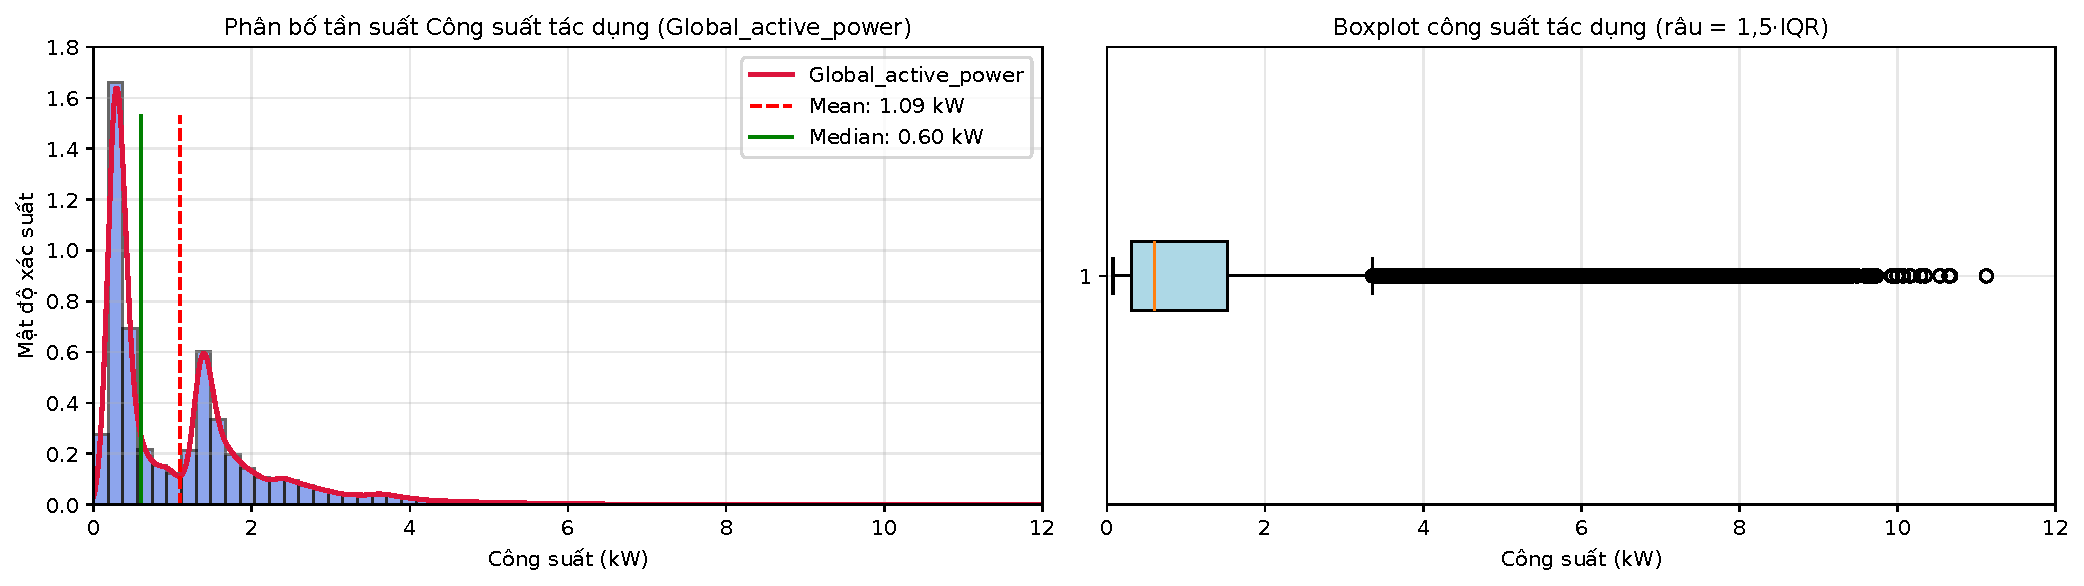
\includegraphics[width=\textwidth]{figures/nb01_gap.pdf}
    \caption{Phân bố công suất tác dụng theo phút: histogram kèm KDE (trái) và biểu đồ hộp với râu 1,5$\cdot$IQR (phải).}
    \label{fig:gap}
\end{figure}

Hình~\ref{fig:gap} cho thấy phân bố công suất lệch phải: khoảng 17,1\% số phút nằm trong vùng tải nền 0,2--0,3 kW. Có 94.907 phút (4,63\%) vượt râu trên 3,358 kW của biểu đồ hộp; đây là các khoảng thời gian tiêu thụ cao kéo dài tới 11,122 kW. Đường KDE tràn nhẹ sang vùng âm là hiệu ứng làm trơn ở biên, không phải dữ liệu âm.

\begin{figure}[htbp]
    \centering
    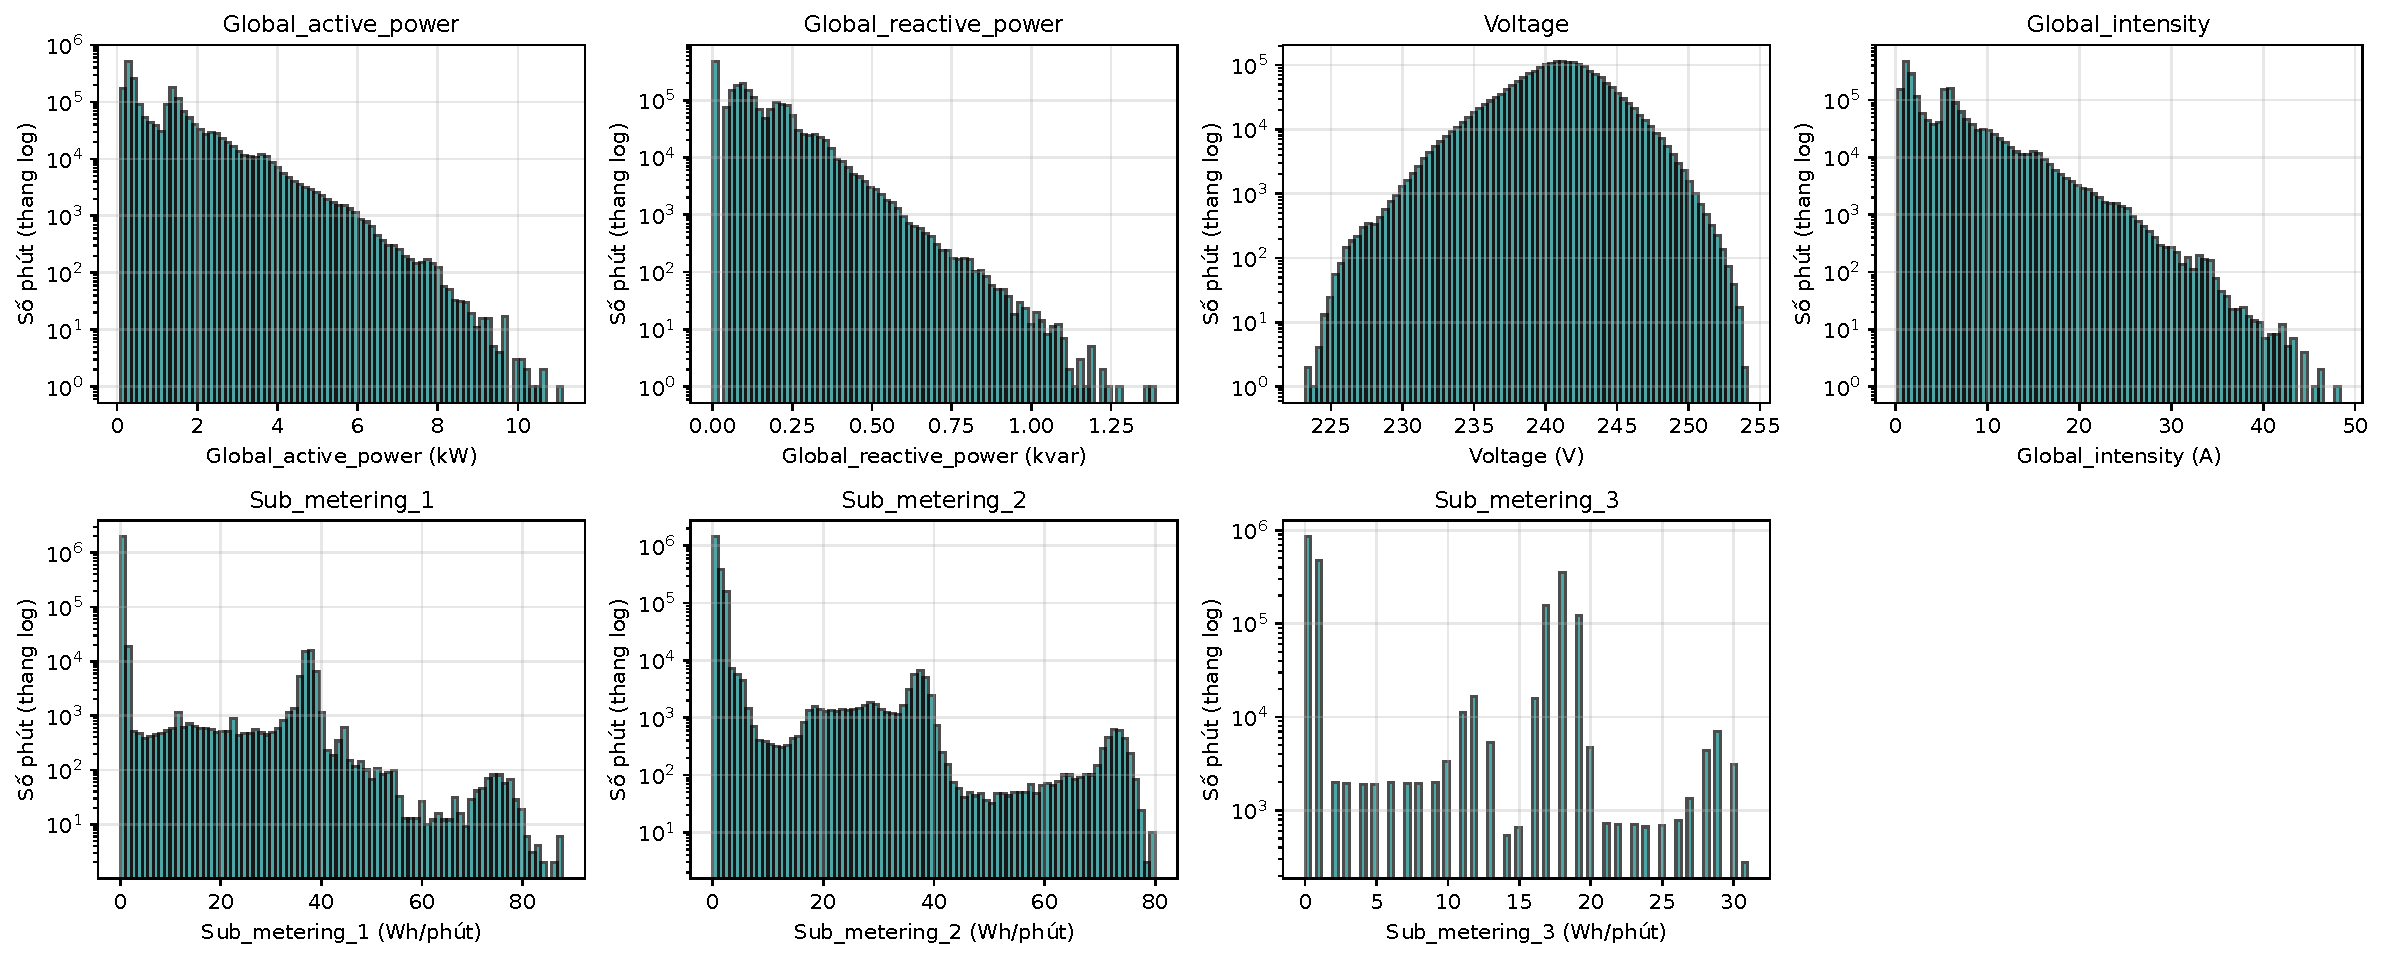
\includegraphics[width=\textwidth]{figures/nb01_bay_bien.pdf}
    \caption{Histogram của bảy biến đo theo phút, trục tung thang logarit.}
    \label{fig:seven}
\end{figure}

Trong Hình~\ref{fig:seven}, công suất tác dụng và cường độ dòng điện có hình dạng gần như giống hệt nhau, là dấu hiệu sớm của tương quan rất cao giữa hai biến. Điện áp có dạng chuông quanh 241 V. \code{Sub_metering_1} và \code{Sub_metering_2} dồn gần hết tại 0, còn \code{Sub_metering_3} có hai cụm tách biệt (0--1 và 17--19 Wh/phút), phù hợp với thiết bị bật/tắt theo bộ ổn nhiệt; đây là giả thuyết vì dữ liệu không cho biết thiết bị nào đang chạy.

\subsection{Nhãn và phân bố nhãn}
\label{sec:label}
Nhãn (điện năng) của một giờ bằng trung bình công suất các phút có đo trong giờ nhân với 1 giờ:
\begin{equation}
    E_{\text{giờ}}\ [\text{kWh}] = \frac{1}{n}\sum_{i=1}^{n} P_i\ [\text{kW}] \times 1\ \text{h},
    \label{eq:energy}
\end{equation}
chỉ tính khi giờ đó có ít nhất 54/60 phút đo; giờ thiếu nhiều hơn được để trống (NaN) và không dùng làm nhãn. Chuỗi theo giờ có 34.589 giờ, trong đó 34.143 giờ hợp lệ (98,71\%). Trên tập huấn luyện (trước 01/01/2010), nhãn có trung bình 1,100 kWh, trung vị 0,794 kWh, độ lệch chuẩn 0,928 kWh và skew 1,31. Phần phân tích phân bố và quan hệ dưới đây chỉ dùng tập huấn luyện để không sử dụng thông tin của tập kiểm tra khi ra quyết định.

\begin{figure}[htbp]
    \centering
    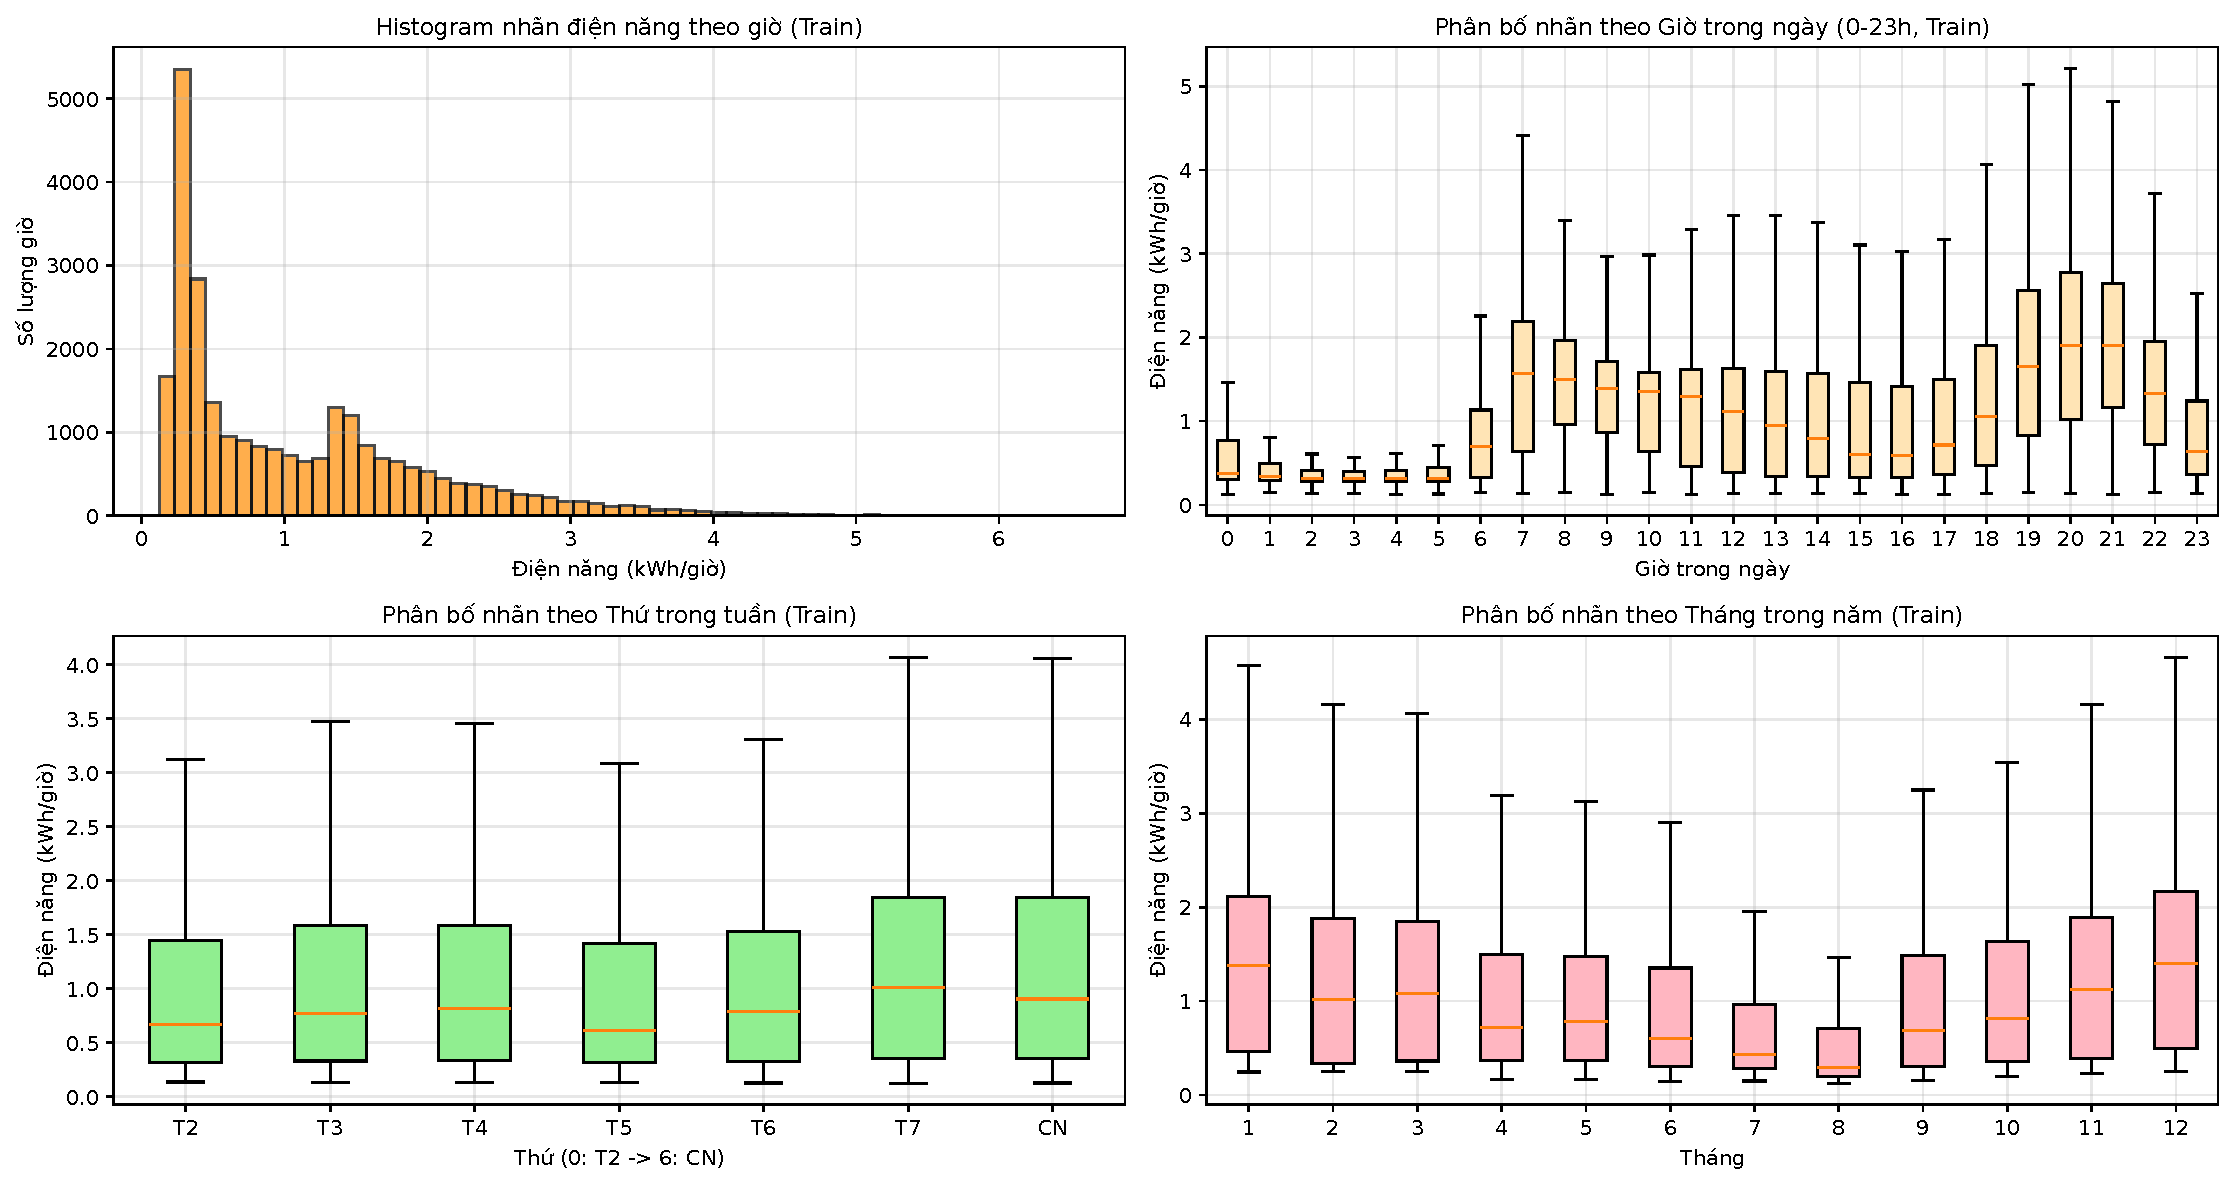
\includegraphics[width=\textwidth]{figures/nb01_nhan.pdf}
    \caption{Phân bố nhãn trên tập huấn luyện: histogram và biểu đồ hộp theo giờ trong ngày, thứ trong tuần, tháng.}
    \label{fig:label}
\end{figure}

Hình~\ref{fig:label} cho thấy bốn đặc điểm của nhãn:
\begin{itemize}
    \item Hai đỉnh: đỉnh chính ở vùng tải nền khoảng 0,23 kWh và đỉnh thứ hai quanh 1,4 kWh.
    \item Chu kỳ ngày: trung vị thấp nhất lúc 3--4 giờ sáng (0,315 kWh), cao nhất lúc 20 giờ (1,904 kWh); khung 19--21 giờ có độ lệch chuẩn lớn nhất (1,10--1,18 kWh), là khung giờ khó dự báo nhất.
    \item Chu kỳ tuần và mùa: trung vị thứ Bảy (1,014) và Chủ nhật (0,904) cao hơn ngày thường (ví dụ thứ Hai 0,665 kWh); tháng 12 cao nhất (1,398 kWh), tháng 8 thấp bất thường (0,289 kWh).
    \item Đuôi phải: chỉ 2,26\% số giờ vượt râu trên 3,494 kWh. Đây là bài toán hồi quy nên không áp dụng cân bằng lớp, nhưng cần theo dõi sai số riêng ở các giờ đỉnh.
\end{itemize}

\subsection{Quan hệ giữa các biến và với nhãn}
\label{sec:correlation}

\begin{figure}[htbp]
    \centering
    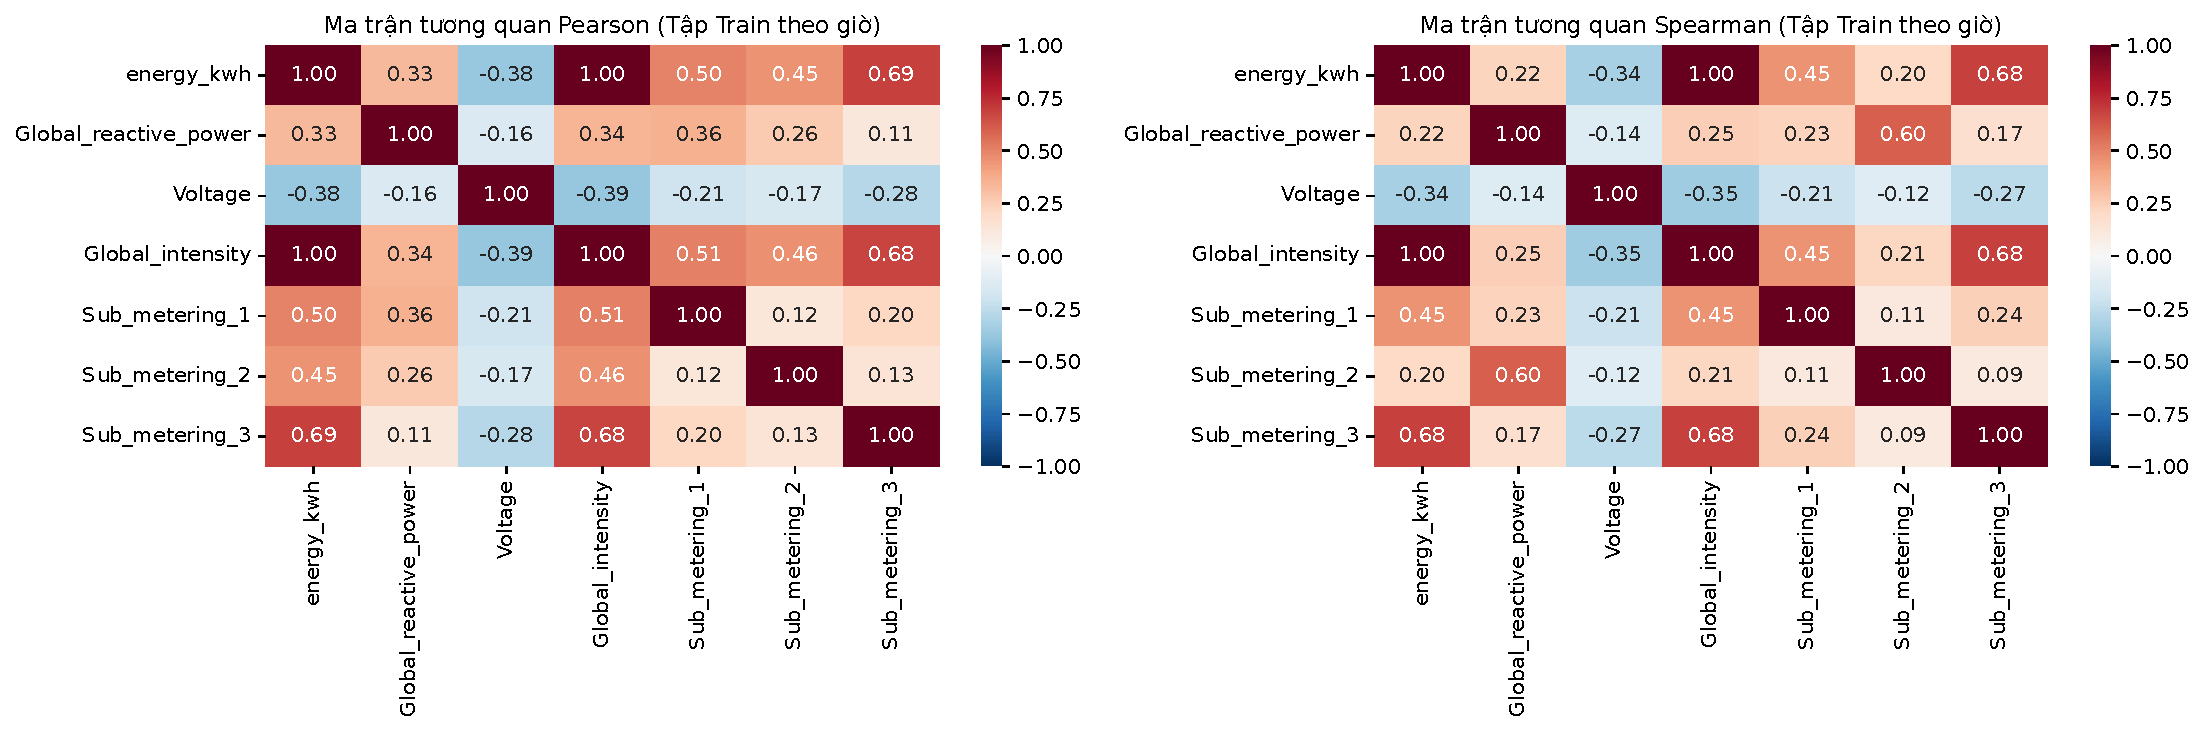
\includegraphics[width=\textwidth]{figures/nb01_tuong_quan.pdf}
    \caption{Ma trận tương quan Pearson (trái) và Spearman (phải) của các biến đo lấy trung bình theo giờ, tập huấn luyện.}
    \label{fig:corr}
\end{figure}

\begin{figure}[htbp]
    \centering
    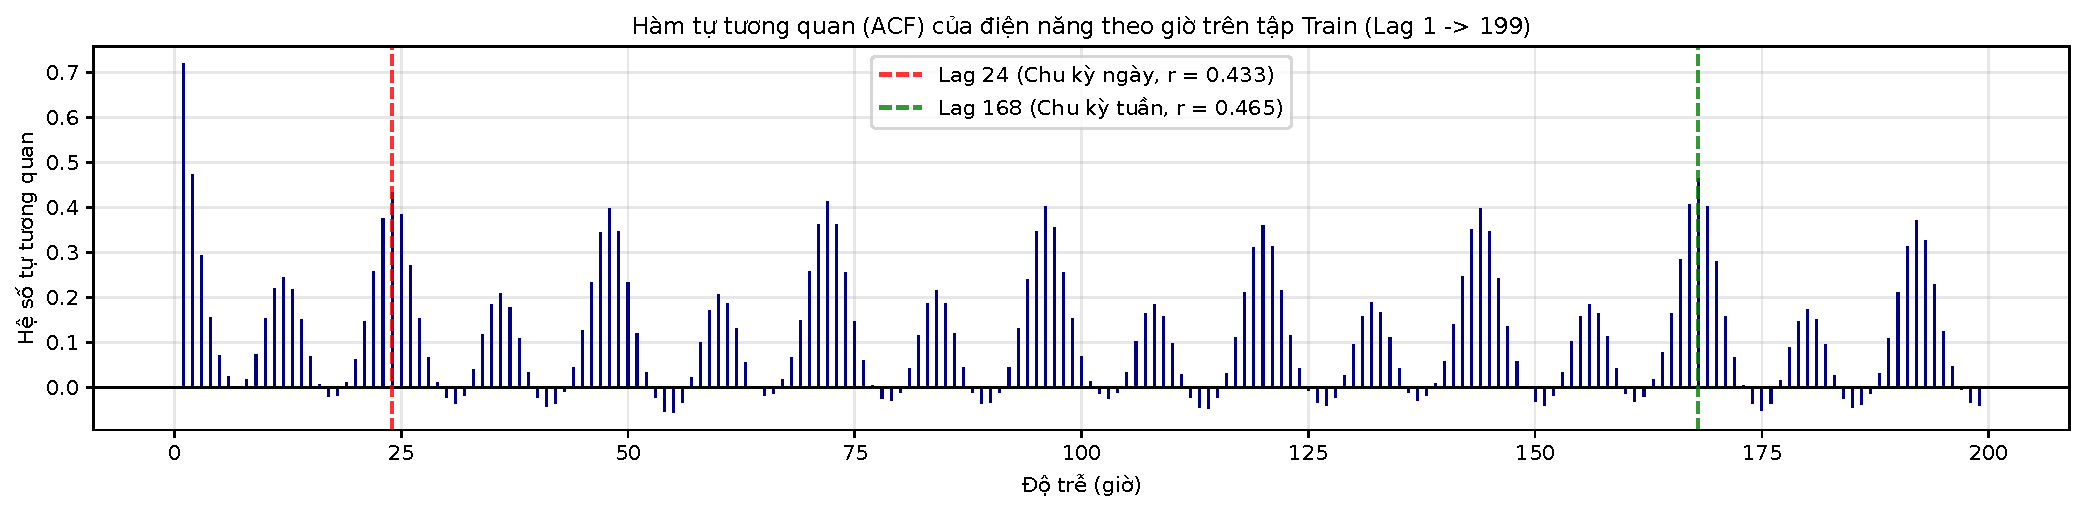
\includegraphics[width=\textwidth]{figures/nb01_acf.pdf}
    \caption{Hàm tự tương quan của điện năng theo giờ trên tập huấn luyện, độ trễ 1--199 giờ.}
    \label{fig:acf}
\end{figure}

Từ Hình~\ref{fig:corr} và Hình~\ref{fig:acf}, nhóm rút ra bốn nhận xét có ý nghĩa cho việc xây dựng mô hình:
\begin{enumerate}
    \item Rò rỉ qua cường độ dòng điện. Tương quan giữa \code{Global_intensity} và nhãn là 0,999 (Pearson) và 0,998 (Spearman), vì công suất xấp xỉ bằng điện áp nhân cường độ. Đại lượng này đo cùng lúc với nhãn nên không có tại thời điểm dự báo; nhóm loại nó, cùng với \code{Voltage} của thời điểm mục tiêu.
    \item Tương quan giảm nhanh rồi tăng lại theo chu kỳ. Tự tương quan giảm từ 0,719 ở độ trễ 1 xuống 0,023 ở độ trễ 6, rồi tăng lại ở 24 giờ (0,433) và 168 giờ (0,465). Vì vậy với $h \ge 6$, thông tin chủ yếu đến từ giá trị cùng giờ ngày trước và tuần trước của thời điểm mục tiêu, không phải từ các giờ gần nhất.
    \item Quan hệ giữa giờ trong ngày và nhãn không đơn điệu (thấp ban đêm, tăng buổi sáng, đỉnh buổi tối). Mô hình tuyến tính cần mã hóa one-hot cho giờ; mô hình cây có thể tự học quan hệ này.
    \item Nhóm công tơ phụ và điện áp. \code{Sub_metering_3} tương quan cao nhất với nhãn trong ba nhóm (0,687) nhưng là giá trị cùng thời điểm, nên chỉ có thể dùng giá trị trễ của nó. Điện áp tương quan âm với nhãn ($-0{,}375$): giờ tiêu thụ cao thường có điện áp thấp hơn.
\end{enumerate}

\subsection{Tính mùa vụ theo ngày}

\begin{figure}[htbp]
    \centering
    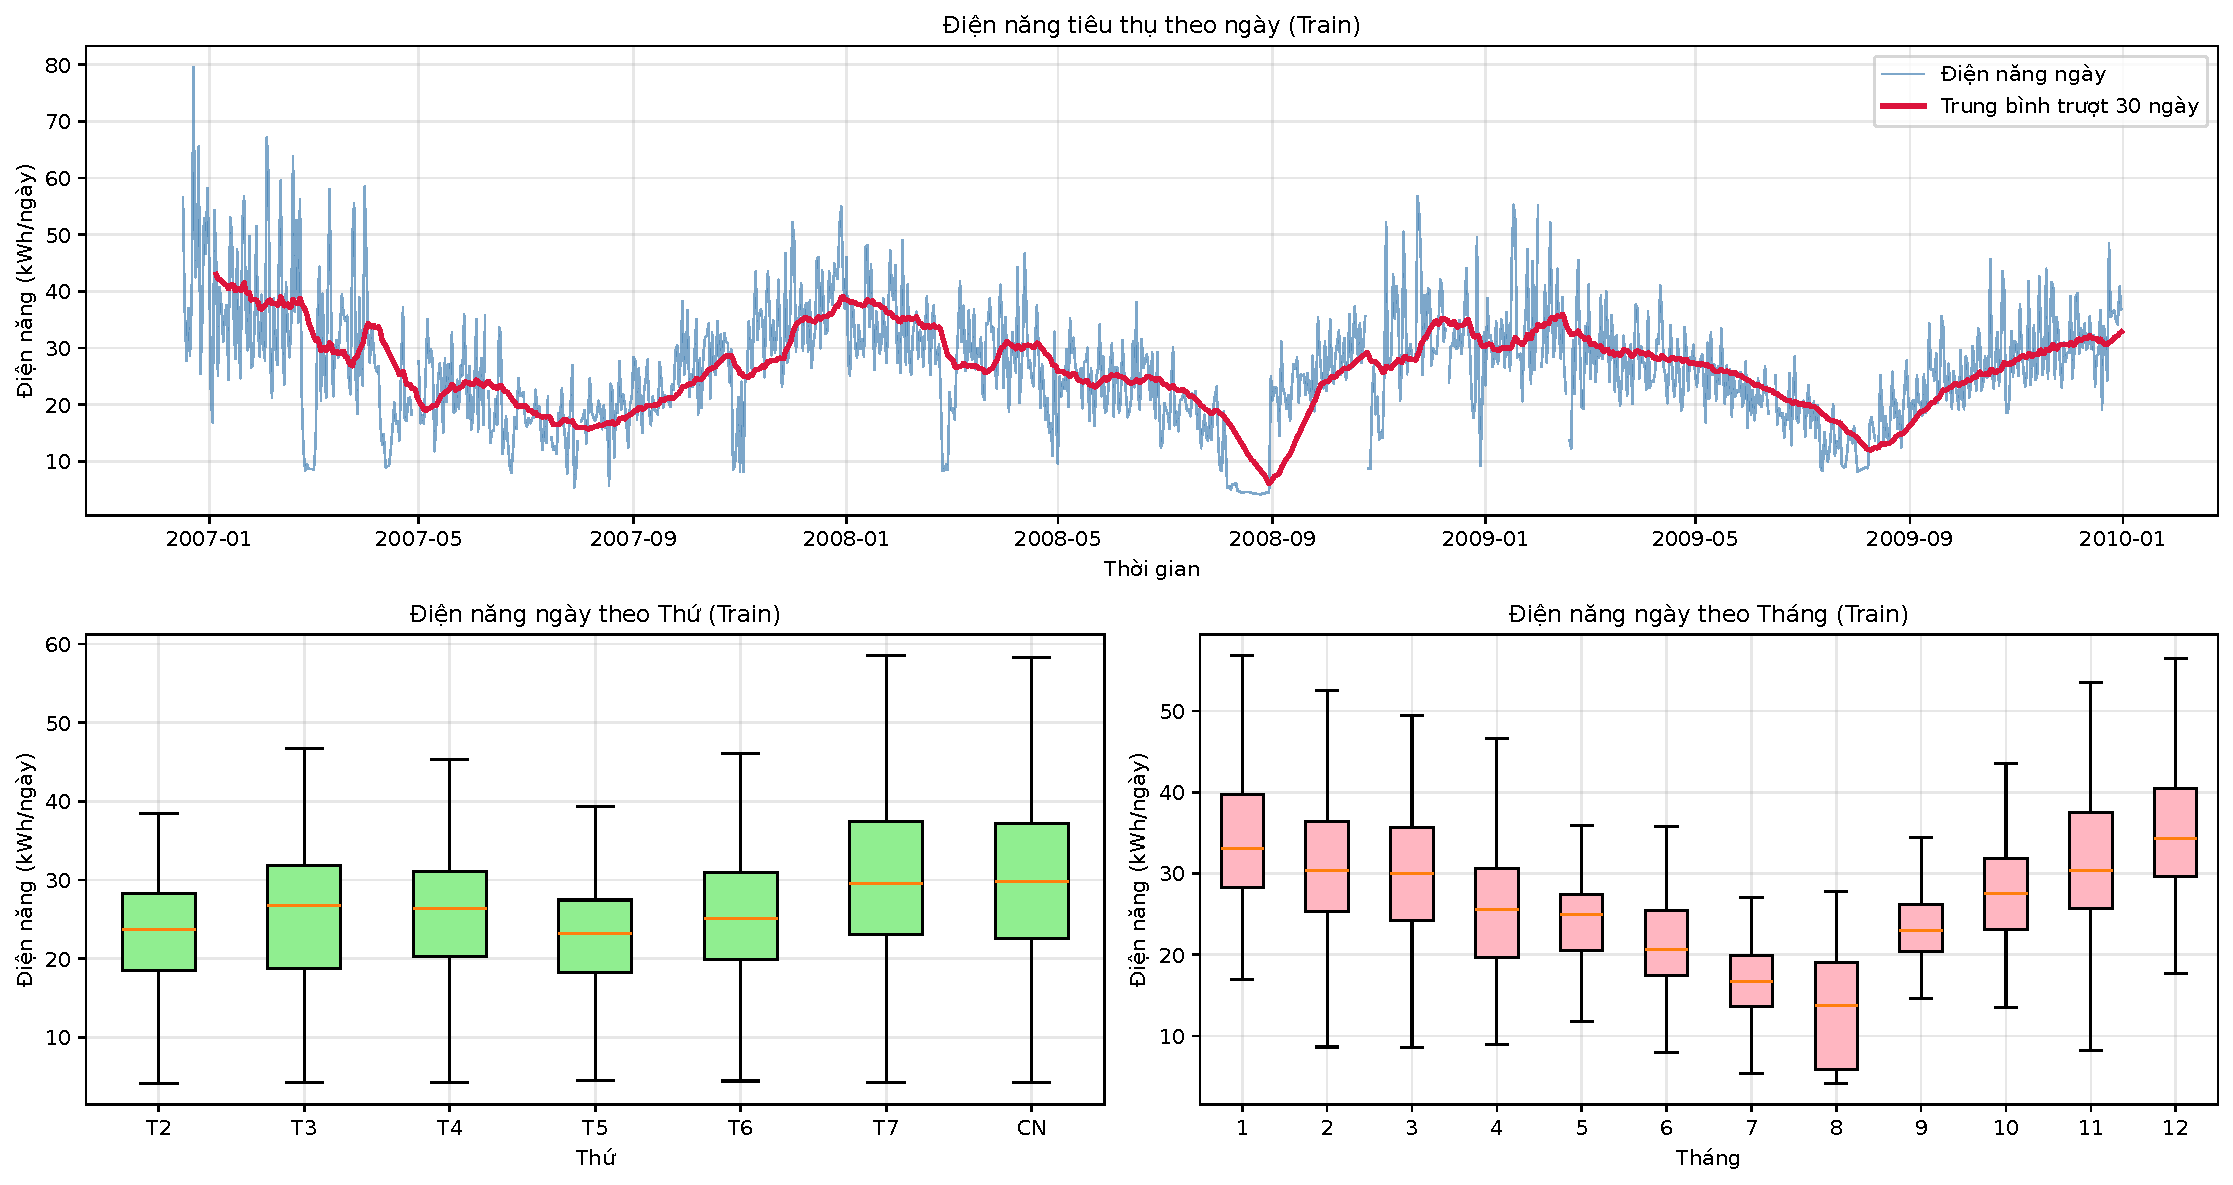
\includegraphics[width=\textwidth]{figures/nb01_theo_ngay.pdf}
    \caption{Điện năng theo ngày trên tập huấn luyện: chuỗi ngày kèm trung bình trượt 30 ngày (trên), biểu đồ hộp theo thứ và theo tháng (dưới).}
    \label{fig:daily}
\end{figure}

Điện năng ngày là tổng 24 giờ; chỉ giữ các ngày đủ 24 giờ hợp lệ (31 trên 1.442 ngày bị loại). Hình~\ref{fig:daily} cho thấy mùa vụ theo năm rõ rệt: trung vị tháng 12 (34,31 kWh/ngày) gấp khoảng 2,5 lần tháng 8 (13,79 kWh/ngày); tự tương quan của chuỗi ngày ở độ trễ 364 ngày là 0,537. Chu kỳ tuần cũng xuất hiện: tự tương quan ở độ trễ 7 ngày (0,554) cao hơn ở 6 ngày (0,499), cuối tuần tiêu thụ cao hơn ngày thường. Nguyên nhân tháng 8 thấp (có thể là kỳ nghỉ hè) không kiểm chứng được từ dữ liệu.

\section{Chất lượng dữ liệu và xử lý}
\label{sec:quality}

\subsection{Định lượng các vấn đề chất lượng}
Bảng~\ref{tab:quality} tổng hợp kết quả kiểm tra chất lượng dữ liệu.

\begin{table}[htbp]
    \centering
    \caption{Các vấn đề chất lượng dữ liệu đã định lượng.}
    \label{tab:quality}
    \small
    \begin{tabularx}{\textwidth}{|>{\raggedright\arraybackslash}p{3.2cm}|>{\raggedright\arraybackslash}X|>{\raggedright\arraybackslash}p{4.0cm}|}
        \hline
        \textbf{Vấn đề} & \textbf{Định lượng} & \textbf{Ảnh hưởng} \\ \hline
        Sai định dạng & 155.874 ký tự ``?'' ở 6 cột số & Cột bị đọc thành chuỗi \\ \hline
        Bản ghi trùng & 0 mốc thời gian trùng; 0 mốc bị thiếu trên lưới 1 phút & Không có \\ \hline
        Giá trị thiếu & 25.979 dòng (1,252\%), cả 25.979 dòng thiếu đồng thời 7 biến & Mất thông tin ở các khoảng thiếu \\ \hline
        Thiếu dạng khối & 71 khối liên tục; 6 khối dài hơn 1 ngày chiếm 94,9\% số phút thiếu; khối dài nhất 120,4 giờ từ 17/08/2010; 4 trong 6 khối dài thuộc năm 2010 & Không phù hợp nội suy; tập kiểm tra bị ảnh hưởng nhiều hơn \\ \hline
        Ngoại lai (1,5$\cdot$IQR) & Công suất: 94.907 phút (4,63\%); \code{Sub_metering_1}: 8,25\% & Là các giờ tiêu thụ cao có thật \\ \hline
        Tính hợp lý vật lý & 0 giá trị âm; 57 phút điện áp trên 253 V (0,003\%) & Không thấy giá trị phi vật lý \\ \hline
        Nhất quán đơn vị & 0,05\% số phút có điện năng ``còn lại'' âm (nhỏ nhất $-2{,}4$ Wh/phút) & Rất nhỏ, có thể do làm tròn \\ \hline
        Nguy cơ rò rỉ & Tương quan giữa công suất và $V \cdot I$ là 0,99909 & Loại \code{Global_intensity} \\ \hline
        Mất cân bằng & 2,26\% số giờ huấn luyện vượt râu trên 3,494 kWh & Theo dõi sai số ở giờ đỉnh \\ \hline
    \end{tabularx}
\end{table}

\begin{figure}[htbp]
    \centering
    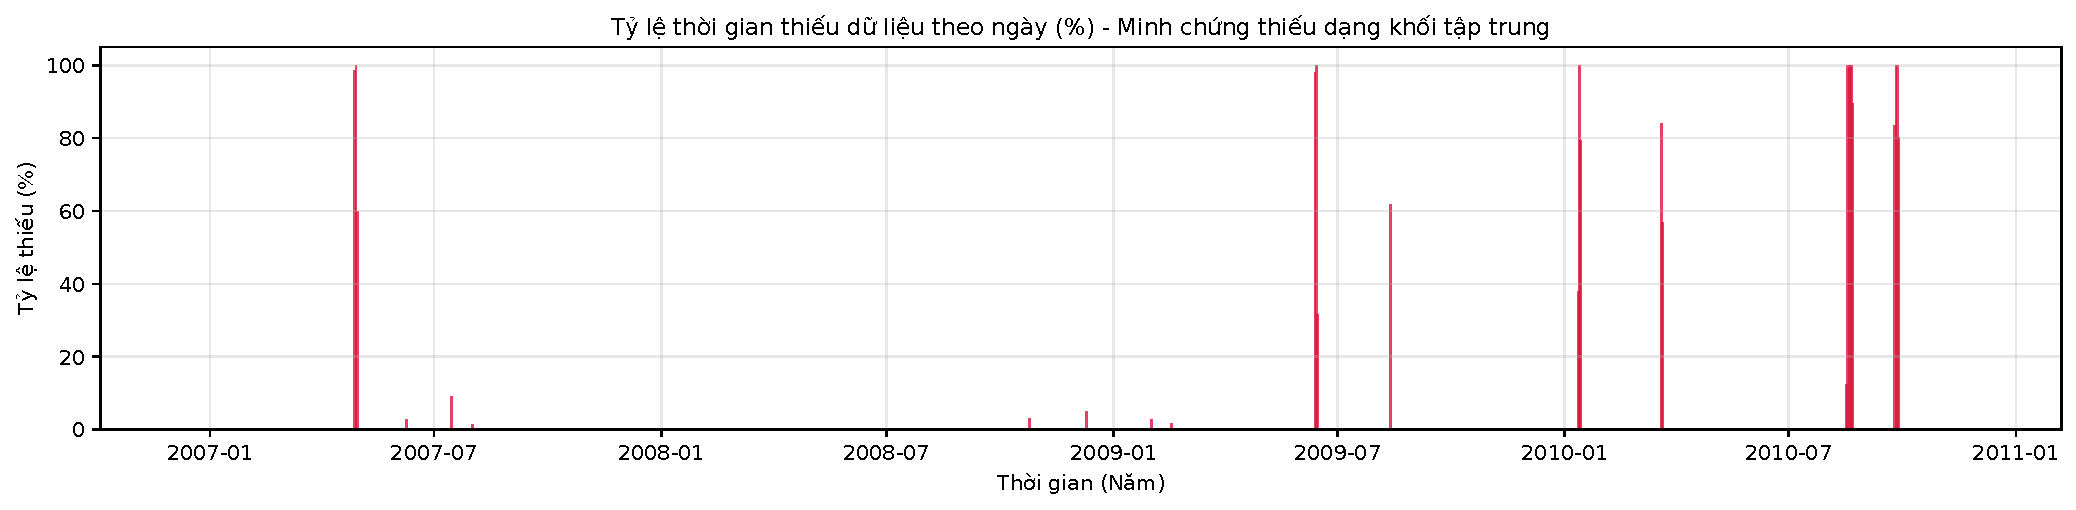
\includegraphics[width=\textwidth]{figures/nb01_thieu_theo_ngay.pdf}
    \caption{Tỷ lệ phút thiếu dữ liệu theo ngày.}
    \label{fig:missing}
\end{figure}

Hình~\ref{fig:missing} cho thấy dữ liệu thiếu không rải rác từng phút mà tập trung thành các khối kéo dài nhiều ngày. Mô hình thiếu này không phù hợp với giả định thiếu hoàn toàn ngẫu nhiên (MCAR)~\cite{little2019statistical}; nguyên nhân có thể là thiết bị ghi bị ngắt, nhưng dữ liệu không cho biết.

\subsection{Phương án xử lý}
Bảng~\ref{tab:treatment} nêu cách xử lý từng vấn đề và lý do lựa chọn.

\begin{table}[htbp]
    \centering
    \caption{Phương án xử lý các vấn đề chất lượng dữ liệu.}
    \label{tab:treatment}
    \small
    \begin{tabularx}{\textwidth}{|>{\raggedright\arraybackslash}p{2.6cm}|>{\raggedright\arraybackslash}p{4.3cm}|>{\raggedright\arraybackslash}X|}
        \hline
        \textbf{Vấn đề} & \textbf{Cách xử lý} & \textbf{Lý do} \\ \hline
        Ký tự ``?'' & Đọc là giá trị thiếu, ép kiểu số thực & ``?'' là ký hiệu thiếu của nguồn; không thay bằng 0 vì hộ luôn có tải nền. \\ \hline
        Thiếu ở nhãn & Tổng hợp theo giờ; giờ có dưới 54 phút đo để NaN; không nội suy, không xóa dòng & Nội suy qua khối thiếu dài tới 5 ngày sẽ tạo nhãn giả từ dữ liệu sau khối. Giữ NaN trên lưới giờ để phép dịch $k$ dòng luôn đúng $k$ giờ. \\ \hline
        Thiếu ở đặc trưng & Điền trung vị trong Pipeline, chỉ học trên tập huấn luyện & Trung vị ít bị kéo bởi giờ đỉnh hơn trung bình khi phân bố lệch phải. \\ \hline
        Ngoại lai & Giữ nguyên & Không có giá trị âm hay vượt ngưỡng vật lý; giờ tiêu thụ cao là đối tượng cần dự báo. \\ \hline
        Rò rỉ & Loại \code{Global_intensity}, \code{Voltage} của thời điểm mục tiêu & Không biết được tại thời điểm dự báo. \\ \hline
        Mất cân bằng & Không sinh mẫu nhân tạo & Sinh mẫu phá vỡ cấu trúc thời gian; thay bằng phân tích sai số theo giờ và theo dải giá trị. \\ \hline
    \end{tabularx}
\end{table}

Ngưỡng 54/60 phút được chọn sau khi thử các ngưỡng khác: đổi ngưỡng từ 60 xuống 1 phút chỉ làm số giờ hợp lệ thay đổi 83 giờ (từ 34.085 lên 34.168), vì phần lớn giờ thiếu là thiếu trọn vẹn (421 giờ không có phút nào). Ngưỡng 54 phút giữ thêm 58 giờ so với ngưỡng 60 mà vẫn bảo đảm trung bình được tính trên ít nhất 90\% thời gian của giờ.

\subsection{So sánh trước và sau xử lý}

\begin{table}[htbp]
    \centering
    \caption{So sánh công suất theo phút (trước) và điện năng theo giờ (sau xử lý).}
    \label{tab:before_after}
    \small
    \begin{tabular}{|l|r|r|}
        \hline
        \textbf{Chỉ số} & \textbf{Trước: công suất theo phút (kW)} & \textbf{Sau: điện năng theo giờ (kWh)} \\ \hline
        Số dòng & 2.075.259 & 34.589 \\ \hline
        Số dòng thiếu (tỷ lệ) & 25.979 (1,252\%) & 446 (1,289\%) \\ \hline
        Trung bình & 1,092 & 1,092 \\ \hline
        Độ lệch chuẩn & 1,057 & 0,898 \\ \hline
        Trung vị & 0,602 & 0,803 \\ \hline
        Min / Max & 0,076 / 11,122 & 0,124 / 6,561 \\ \hline
        Skew & 1,79 & 1,30 \\ \hline
    \end{tabular}
\end{table}

\begin{figure}[htbp]
    \centering
    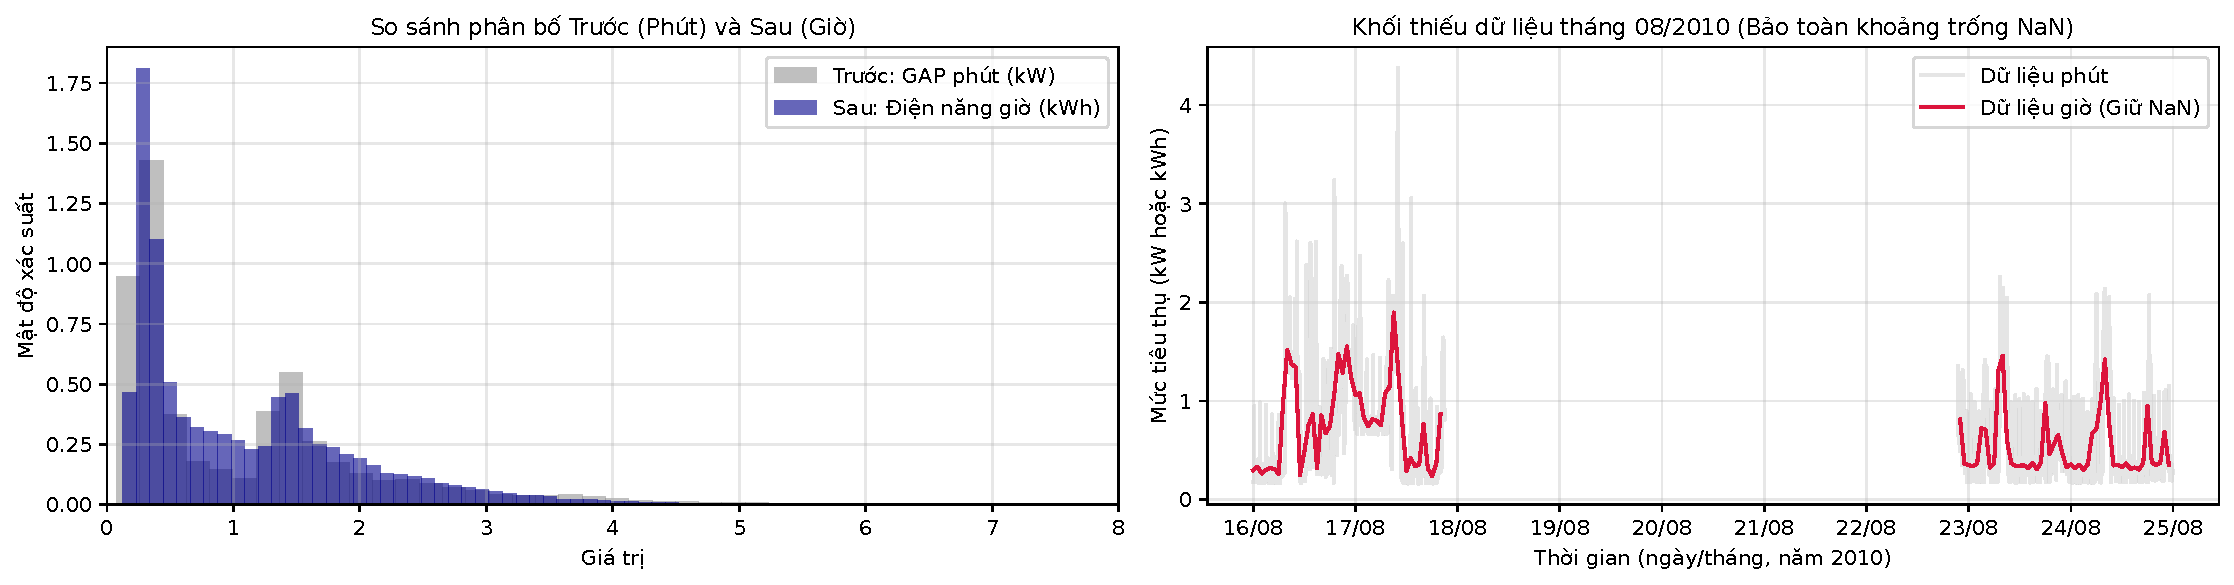
\includegraphics[width=\textwidth]{figures/nb01_truoc_sau.pdf}
    \caption{Phân bố trước và sau xử lý (trái); đoạn chứa khối thiếu dài nhất tháng 8/2010, khối thiếu được giữ nguyên (phải).}
    \label{fig:before_after}
\end{figure}

Bảng~\ref{tab:before_after} và Hình~\ref{fig:before_after} cho thấy trung bình giữ nguyên 1,092 (điện năng được bảo toàn khi gộp theo giờ), còn độ lệch chuẩn giảm 15\%, giá trị lớn nhất giảm từ 11,122 xuống 6,561 và skew giảm từ 1,79 xuống 1,30, do các đỉnh kéo dài vài phút được trung bình hóa trong giờ. Khối thiếu tháng 8/2010 được để trống thay vì nối bằng một đoạn thẳng giả.

\section{Chuẩn bị dữ liệu cho mô hình}
\label{sec:preparation}

\subsection{Chia dữ liệu theo thời gian}
Dữ liệu được chia theo thời điểm mục tiêu $t+h$, không xáo trộn: mẫu có nhãn trước 01/01/2010 thuộc tập huấn luyện, từ 01/01/2010 thuộc tập kiểm tra. Chia theo thời điểm mục tiêu (thay vì thời điểm gốc) bảo đảm không có nhãn nào của năm 2010 lọt vào tập huấn luyện, kể cả khi $h = 24$. Với $h = 1$, tập huấn luyện có 26.523 mẫu (nhãn từ 16/12/2006 đến 31/12/2009, 77,7\%) và tập kiểm tra có 7.620 mẫu (từ 01/01/2010 đến 26/11/2010, 22,3\%). Tập kiểm tra được giữ riêng: không dùng để khảo sát, chọn đặc trưng hay chọn mô hình.

\subsection{Kiểm định chéo theo thời gian}
Trên tập huấn luyện, nhóm dùng TimeSeriesSplit với 5 fold, mỗi fold kiểm định dài 2.160 giờ (90 ngày) và khoảng đệm 168 mẫu (một tuần) giữa phần huấn luyện và phần kiểm định~\cite{sklearn2026tss}.

\begin{table}[htbp]
    \centering
    \caption{Các fold kiểm định chéo với $h = 1$ (mọi fold huấn luyện bắt đầu từ 16/12/2006).}
    \label{tab:folds}
    \small
    \begin{tabular}{|c|r|c|r|c|}
        \hline
        \textbf{Fold} & \textbf{Mẫu huấn luyện} & \textbf{Huấn luyện đến} & \textbf{Mẫu kiểm định} & \textbf{Khoảng kiểm định} \\ \hline
        1 & 15.555 & 27/09/2008 & 2.160 & 04/10/2008 -- 02/01/2009 \\ \hline
        2 & 17.715 & 26/12/2008 & 2.160 & 02/01/2009 -- 03/04/2009 \\ \hline
        3 & 19.875 & 27/03/2009 & 2.160 & 03/04/2009 -- 04/07/2009 \\ \hline
        4 & 22.035 & 27/06/2009 & 2.160 & 04/07/2009 -- 02/10/2009 \\ \hline
        5 & 24.195 & 25/09/2009 & 2.160 & 03/10/2009 -- 31/12/2009 \\ \hline
    \end{tabular}
\end{table}

\begin{figure}[htbp]
    \centering
    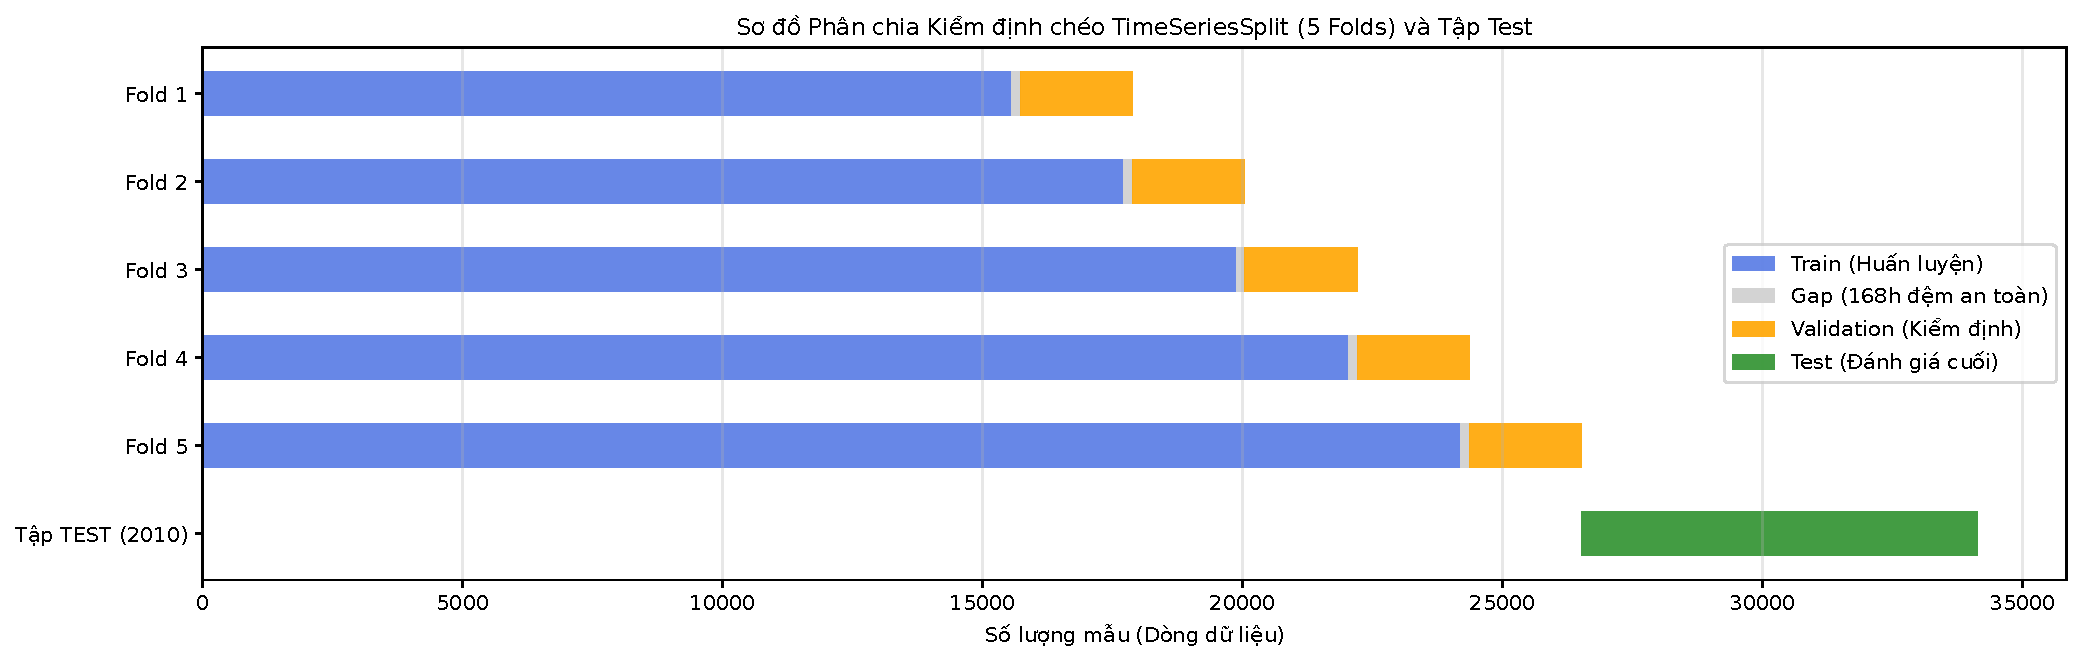
\includegraphics[width=\textwidth]{figures/nb02_fold.pdf}
    \caption{Sơ đồ 5 fold TimeSeriesSplit và tập kiểm tra; trục hoành là chỉ số mẫu.}
    \label{fig:folds}
\end{figure}

Như Bảng~\ref{tab:folds} và Hình~\ref{fig:folds}, các fold kiểm định có cùng kích thước, nối tiếp và không chồng nhau; phần huấn luyện mở rộng thêm 2.160 mẫu mỗi fold. Khoảng đệm bảo đảm nhãn của các mẫu huấn luyện cuối cùng không trùng khoảng thời gian với nhãn của các mẫu kiểm định đầu tiên khi $h \le 24$, đồng thời giảm phụ thuộc do tự tương quan giữa hai phần. Các fold kiểm định rơi vào các mùa khác nhau, nên chênh lệch sai số giữa các fold phản ánh cả mùa vụ; kết quả vì vậy được báo cáo bằng trung bình $\pm$ độ lệch chuẩn qua 5 fold.

\subsection{Đường ống tiền xử lý}
Các bước tiền xử lý được tổ chức thành một Pipeline của thư viện scikit-learn~\cite{pedregosa2011scikit}: biến giờ trong ngày được mã hóa one-hot, các đặc trưng số được điền khuyết bằng trung vị rồi chuẩn hóa z-score. Đường ống chỉ được khớp (fit) trên dữ liệu huấn luyện; với $h = 1$, giá trị học được cho đặc trưng $y_t$ là trung vị 0,7939, trung bình 1,1002 và độ lệch chuẩn 0,9278 kWh.

\begin{figure}[htbp]
    \centering
    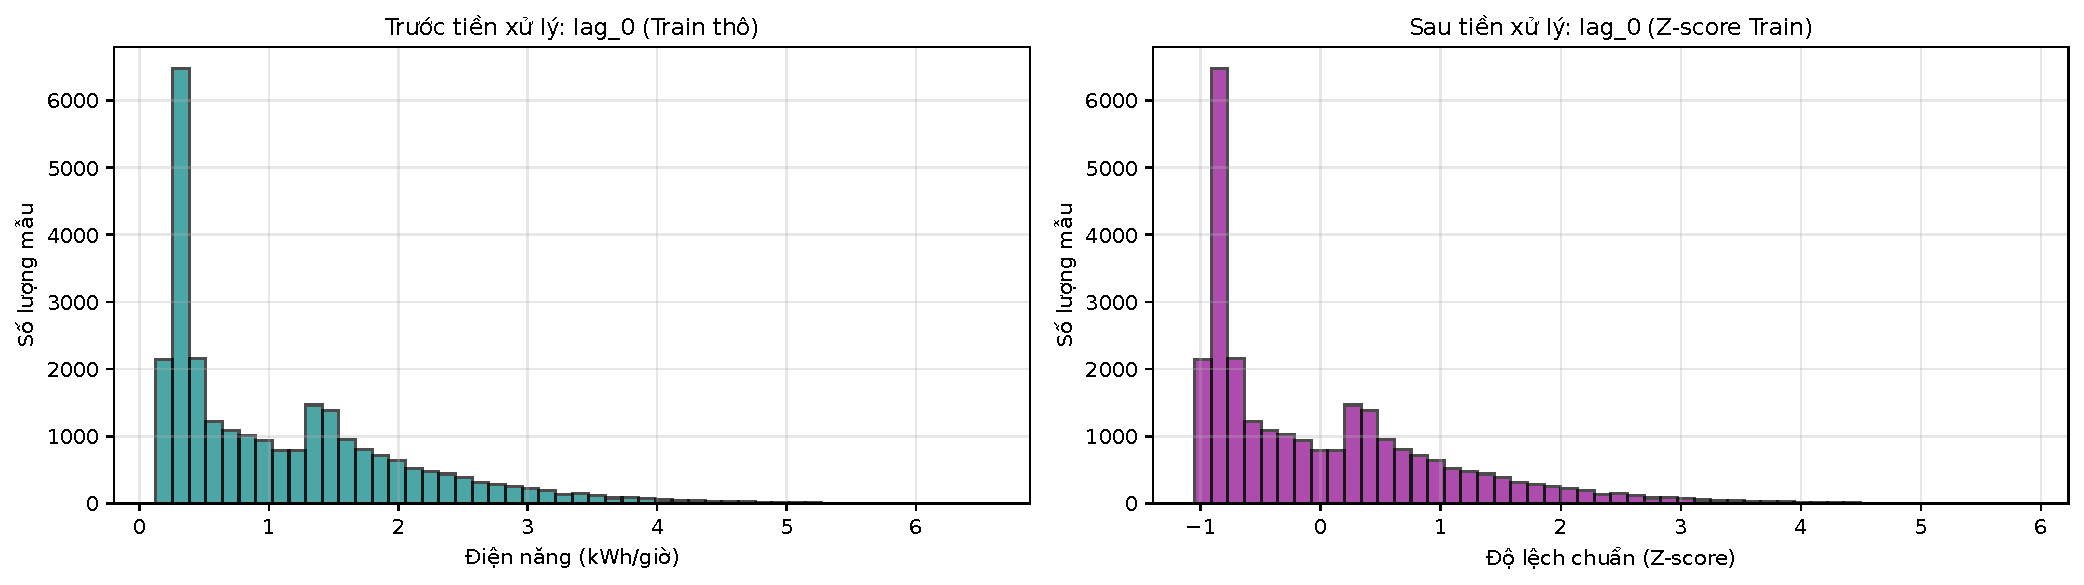
\includegraphics[width=\textwidth]{figures/nb02_chuan_hoa.pdf}
    \caption{Phân bố của đặc trưng $y_t$ trên tập huấn luyện trước và sau tiền xử lý.}
    \label{fig:scaling}
\end{figure}

Sau tiền xử lý, số giá trị thiếu ở cả hai tập về 0. Trên tập huấn luyện, các đặc trưng số có trung bình 0 và độ lệch chuẩn 1; trên tập kiểm tra, trung bình khoảng $-0{,}04$ và độ lệch chuẩn khoảng 0,84, vì năm 2010 tiêu thụ thấp và ít biến động hơn giai đoạn huấn luyện. Điều này cho thấy tập kiểm tra không bị dùng để học tham số chuẩn hóa. Hình~\ref{fig:scaling} cho thấy chuẩn hóa chỉ dịch và co giãn trục, không đổi hình dạng phân bố. Để minh họa rò rỉ, nhóm so sánh với cách khớp trên toàn bộ dữ liệu: trung bình học được của $y_t$ giảm từ 1,1004 xuống 1,0916 và độ lệch chuẩn giảm khoảng 0,03, tức thông tin của năm 2010 đã lọt vào tham số chuẩn hóa.
